
\section{Optimizing the Monitoring Topology}\label{sec:ecmpfree-algo}

\begin{definition}
A graph weight function is said to be \emph{complete} if every link belongs to some shortest path.
\end{definition}

\begin{definition}
A graph weight function is said to be \emph{ECMP-free} if there exists a single shortest path
between any pair of nodes.
\end{definition}

Figure \ref{fig:nonSP} shows a cumulative distribution over all topologies of the percentage of
edges that do not belong to any shortest path. We see that most topologies have some percentage of edges
that no not belong to shortest paths, meaning that their IGP weight functions are not complete. Tipically, but not always, these
edges correspond to backup links with high IGP weights configured on them.
This implies that in order to be able to have a full coverage of the network links using cycles we have two options:

\begin{enumerate}[i)]
 \item Compute a set of IGP weights that is complete and use these weights for the monitoring.
 \item Use adjacency segments to cover these links.
\end{enumerate}

We study both options and analyse their tade-offs.


\begin{figure}
\begin{center}
\includegraphics[width=.85\columnwidth]{./Network-lib/data/plot/nonSP.eps}
\end{center}
\caption{Cumulative distribution of the percentage of edges that no not belong to any shortest path across all topologies.}
\label{fig:nonSP}
\end{figure}




We propose an algorithm to compute IGP weights for the monitoring topology (only used for monitoring) so that
\begin{enumerate}
 \item every link belongs to some shortest path,
 \item there is as few ECMP paths as possible.
\end{enumerate}
%Given the first condition, we know that, except for parallel links, every link can
%be traversed using only node segments.

Let $p_i$ be the $i$-th prime number. Let $m$ denote the number of edges in the network and let $\mathcal{P}_m = \{ p_1, p_2, \ldots, p_m \}$ be the set of
the first $m$ prime numbers.

The key idea of the algorithm is to use the logarithm of these prime numbers as IGP weights.
Indeed, these weights would guarantee that any two paths have a distinct cost, since $\ln(x) + \ln(y) = \ln(x \cdot y)$
and $\ln$ is injective. Thus, the cost of the first path is the logarithm of some product of prime numbers whereas the weight of the second
path is the logarithm of the product of some other prime numbers. Since these products are distinct, their logarithms must
also be distinct. %Unfortunatelly we cannot use these weights as is since they are real numbers.

Since the IGP weights must be integers, we use a truncated logarithm $\overline{\ln}^s$, defined as follows:
$$
\overline{\ln}^s(x) = \lfloor 10^s \cdot \ln(x) \rfloor
$$
For instance, $\overline{\ln}^4(5) = \lfloor 10^4 \cdot 1.60943... \rfloor = 16094$.
The next proposition studies how the sums of truncated logarithms behave when $s$
increases. This is important to prove that our algorithm will eventually find
weights without ECMP.
%In our algorithm, we start with $s = 0$ and increase $s$ until there is no ECMP.
%The following proposition proves that the algorithm finds a solution in a finite
%number of iterations.
% \begin{lemma}
% $$
% \log(x \cdot y) \geq \overline{\log}(x) + \overline{\log}(y)
% $$
% \end{lemma}
% \begin{proof}
% $$
% \log(x \cdot y) = \log(x) + \log(y) 
% $$
% the result follows since $\log(x) \geq \overline{\log}(x)$.
% \end{proof}
% \begin{lemma}
% $$
% \overline{\log}(x) + \overline{\log}(y) \geq \log(x \cdot y) - 2 \cdot 10^{-k}
% $$
% \end{lemma}
% \begin{proof}
% We have
% $$
% \overline{\log}(x) = \frac{\lfloor 10^k \cdot \log(x) \rfloor}{10^k} \geq \frac{10^k \cdot \log(x) - 1}{10^k} = \log(x) - 10^{-k}.
% $$
% Hence
% $$
% \overline{\log}(x) + \overline{\log}(y) \geq \log(x) - 10^{-k} + \log(y) - 10^{-k} = \log(x \cdot y) - 2 \cdot 10^{-k}
% $$
% \end{proof}
% It follows immediatily from the two previous lemma that in general,

\begin{proposition}
\label{prop:converge}
Let $A$ and $B$ be two distinct subsets of $\mathcal{P}_m$, $P = \prod_{x \in \mathcal{P}_x} x$ and $q \in \mathcal{P}_m$. If $s > \log_{10} \left( 2 m \cdot q^m P \right)$, 
then $\sum_{x \in A} \left( \overline{\ln}^s(x) + \overline{\ln}^s(q) \right) \neq \sum_{x \in B} \left( \overline{\ln}^s(x) + \overline{\ln}^s(q) \right)$.
\end{proposition}

\begin{proof}
Given any $s$ and $X \subseteq \mathcal{P}_m$, we have
\begin{equation}
\small
\label{eq:lg}
10^s \cdot \ln \left( \prod_{x \in X} x \right) \geq \sum_{x \in X} \overline{\ln}^s(x) \geq 10^s \cdot \ln \left( \prod_{x \in X} x \right) - |X|
\end{equation}

Let $q \in \mathcal{P}_m$. Write $a = \prod_{x \in A} x$ and $b = \prod_{x \in B} x$. Assume without loss of generality that $q^{|A|} a > q^{|B|} b$ (they are not equal because they contain distinct prime numbers). 
Then by (\ref{eq:lg})
\begin{align*}
\tiny
\sum_{x \in A} \overline{\ln}^s(x) +  \overline{\ln}^s(q) & \geq \sum_{x \in A} 10^s \ln(x q) - 2 \geq \\
& 10^s \ln(q^{|A|} a) - 2 |A|
\end{align*}
and $\sum_{x \in B} \overline{\ln}^s(x) + \overline{\ln}^s(q) \leq 10^s \ln (q^{|B|} b)$. Therefore
\begin{align*}
\tiny
\sum_{x \in A} \overline{\ln}^s(x) +  \overline{\ln}^s(q) - \sum_{x \in B} \overline{\ln}^s(x) + \overline{\ln}^s(q) & \geq \\
10^s \ln(q^{|A|} a) - 2 |A| - 10^s \ln (q^{|B|} b) & \geq \\
10^s  \ln \left(q^{|A|} a \slash q^{|B|} b \right) - 2 |A| \geq & \\
10^s  \ln \left(q^{|A|} a \slash (q^{|A|} a - 1) \right) - 2 |A| \geq & \\
10^s \slash (q^{|A|} a) - 2|A| \geq 10^s \slash (q^m P) - 2m
\end{align*}
Which is positive as long as $s > \log_{10} \left( 2 m \cdot q^m P \right)$.
\end{proof}

%Proposition \ref{prop:converge} says that, after a finite number of iterations, we find weights such that no two paths have the same
%cost. However, this does not guarantee that every edge belongs to a shortest path.

Proposition \ref{prop:converge} shows that for any choice of $q$, if we assign a prime number $p_e$ to each edge 
$e$ and define $w(e) = \overline{\ln}^s(p_e) + \overline{\ln}^s(q)$ then, if $s$ is
large enough, no two paths have the same cost. Since we only require that no two 
shortest paths have the same cost, in practice, a much smaller $s$ will work.

Further, if $q = p_m$ then $q \geq p_e$ for all $e$ so that these weights ensure that $e = (v, u)$ is the shortest path between $v$ and $u$.
\begin{proof}
Let $P$ be any other path from $v$ to $u$. Then $|P| \geq 2$ and
\begin{align*}
\tiny
w(P) & = |P| \cdot \overline{\ln}^s(q) + \sum_{e \in E(P)} \overline{\ln}^s(p_e) > |P| \cdot \overline{\ln}^s(q) \geq \\
& 2 \cdot \overline{\ln}^s(q) \geq \overline{\ln}^s(p_e) + \overline{\ln}^s(q) = w(e)
\end{align*}
\end{proof}

Thus, our algorithm to compute the IGP weights for the monitoring topology
consists in $(i)$ computing the first $m$ prime numbers and identifying each
of them with an edge, $(ii)$ setting $w(e) = \overline{\ln}^s(p_e) + \overline{\ln}^s(p_m)$ and
iterating over $s$ until no two shortest paths have the same weight.

\begin{figure}


\begin{center}
\begin{tabular}{c c c}

&

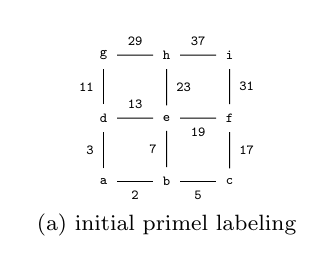
\begin{tikzpicture}[scale = 0.8]
\def\dx{0} 
\def\dy{0} 

\node[font=\bf] (a) at (\dx, \dy) {\tiny \texttt{a}};
\node[font=\bf] (b) at (\dx + 1, \dy) {\tiny \texttt{b}};
\node[font=\bf] (c) at (\dx + 2, \dy) {\tiny \texttt{c}};
\node[font=\bf] (d) at (\dx, \dy + 1) {\tiny \texttt{d}};
\node[font=\bf] (e) at (\dx + 1, \dy + 1) {\tiny \texttt{e}};
\node[font=\bf] (f) at (\dx + 2, \dy + 1) {\tiny \texttt{f}};
\node[font=\bf] (g) at (\dx, \dy + 2) {\tiny \texttt{g}};
\node[font=\bf] (h) at (\dx + 1, \dy + 2) {\tiny \texttt{h}};
\node[font=\bf] (i) at (\dx + 2, \dy + 2) {\tiny \texttt{i}};

\draw (a) edge[] node[anchor = north, font=\bf] {\tiny \texttt{2}}  (b);
\draw (a) edge[] node[anchor = east, font=\bf]  {\tiny \texttt{3}}  (d);
\draw (b) edge[] node[anchor = north, font=\bf] {\tiny \texttt{5}}  (c);
\draw (b) edge[] node[anchor = east, font=\bf]  {\tiny \texttt{7}}  (e);
\draw (d) edge[] node[anchor = east, font=\bf]  {\tiny \texttt{11}} (g);
\draw (d) edge[] node[anchor = south, font=\bf]  {\tiny \texttt{13}} (e);
\draw (c) edge[] node[anchor = west, font=\bf]  {\tiny \texttt{17}} (f);
\draw (e) edge[] node[anchor = north, font=\bf] {\tiny \texttt{19}} (f);
\draw (e) edge[] node[anchor = west, font=\bf]  {\tiny \texttt{23}} (h);
\draw (g) edge[] node[anchor = south, font=\bf]  {\tiny \texttt{29}} (h);
\draw (f) edge[] node[anchor = west, font=\bf] {\tiny \texttt{31}} (i);
\draw (h) edge[] node[anchor = south, font=\bf] {\tiny \texttt{37}} (i);
\node at (1, -0.7) {\footnotesize (a) initial primel labeling};
\end{tikzpicture} 

&

\\

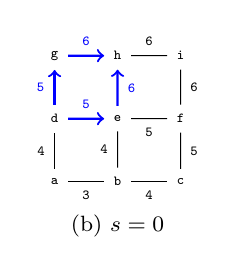
\begin{tikzpicture}[scale = 0.8]
\def\dx{0} 
\def\dy{0} 

\node[font=\bf] (a) at (\dx, \dy) {\tiny \texttt{a}};
\node[font=\bf] (b) at (\dx + 1, \dy) {\tiny \texttt{b}};
\node[font=\bf] (c) at (\dx + 2, \dy) {\tiny \texttt{c}};
\node[font=\bf] (d) at (\dx, \dy + 1) {\tiny \texttt{d}};
\node[font=\bf] (e) at (\dx + 1, \dy + 1) {\tiny \texttt{e}};
\node[font=\bf] (f) at (\dx + 2, \dy + 1) {\tiny \texttt{f}};
\node[font=\bf] (g) at (\dx, \dy + 2) {\tiny \texttt{g}};
\node[font=\bf] (h) at (\dx + 1, \dy + 2) {\tiny \texttt{h}};
\node[font=\bf] (i) at (\dx + 2, \dy + 2) {\tiny \texttt{i}};

\draw (a) edge[] node[anchor = north, font=\bf] {\tiny \texttt{3}} (b);
\draw (a) edge[] node[anchor = east, font=\bf]  {\tiny \texttt{4}} (d);
\draw (b) edge[] node[anchor = north, font=\bf] {\tiny \texttt{4}} (c);
\draw (b) edge[] node[anchor = east, font=\bf]  {\tiny \texttt{4}} (e);
\draw (d) edge[blue, ->, thick] node[anchor = east, font=\bf] {\tiny \texttt{5}} (g);
\draw (d) edge[blue, ->, thick] node[anchor = south, font=\bf]  {\tiny \texttt{5}} (e);
\draw (c) edge[] node[anchor = west, font=\bf]  {\tiny \texttt{5}} (f);
\draw (e) edge[] node[anchor = north, font=\bf] {\tiny \texttt{5}} (f);
\draw (e) edge[blue, ->, thick] node[anchor = west, font=\bf]  {\tiny \texttt{6}} (h);
\draw (g) edge[blue, ->, thick] node[anchor = south, font=\bf] {\tiny \texttt{6}} (h);
\draw (f) edge[] node[anchor = west, font=\bf]  {\tiny \texttt{6}} (i);
\draw (h) edge[] node[anchor = south, font=\bf] {\tiny \texttt{6}} (i);
\node at (1, -0.7) {\footnotesize (b) $s = 0$};
\end{tikzpicture}

&

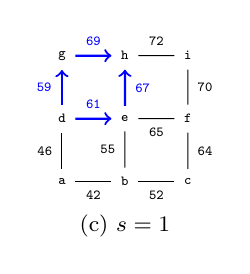
\begin{tikzpicture}[scale = 0.8]
\def\dx{0} 
\def\dy{0} 

\node[font=\bf] (a) at (\dx, \dy) {\tiny \texttt{a}};
\node[font=\bf] (b) at (\dx + 1, \dy) {\tiny \texttt{b}};
\node[font=\bf] (c) at (\dx + 2, \dy) {\tiny \texttt{c}};
\node[font=\bf] (d) at (\dx, \dy + 1) {\tiny \texttt{d}};
\node[font=\bf] (e) at (\dx + 1, \dy + 1) {\tiny \texttt{e}};
\node[font=\bf] (f) at (\dx + 2, \dy + 1) {\tiny \texttt{f}};
\node[font=\bf] (g) at (\dx, \dy + 2) {\tiny \texttt{g}};
\node[font=\bf] (h) at (\dx + 1, \dy + 2) {\tiny \texttt{h}};
\node[font=\bf] (i) at (\dx + 2, \dy + 2) {\tiny \texttt{i}};

\draw (a) edge[] node[anchor = north, font=\bf] {\tiny \texttt{42}} (b);
\draw (a) edge[] node[anchor = east, font=\bf]  {\tiny \texttt{46}} (d);
\draw (b) edge[] node[anchor = north, font=\bf] {\tiny \texttt{52}} (c);
\draw (b) edge[] node[anchor = east, font=\bf]  {\tiny \texttt{55}} (e);
\draw (d) edge[blue, ->, thick] node[anchor = east, font=\bf] {\tiny \texttt{59}} (g);
\draw (d) edge[blue, ->, thick] node[anchor = south, font=\bf]  {\tiny \texttt{61}} (e);
\draw (c) edge[] node[anchor = west, font=\bf]  {\tiny \texttt{64}} (f);
\draw (e) edge[] node[anchor = north, font=\bf] {\tiny \texttt{65}} (f);
\draw (e) edge[blue, ->, thick] node[anchor = west, font=\bf]  {\tiny \texttt{67}} (h);
\draw (g) edge[blue, ->, thick] node[anchor = south, font=\bf] {\tiny \texttt{69}} (h);
\draw (f) edge[] node[anchor = west, font=\bf]  {\tiny \texttt{70}} (i);
\draw (h) edge[] node[anchor = south, font=\bf] {\tiny \texttt{72}} (i);

\node at (1, -0.7) {\footnotesize (c) $s = 1$};
\end{tikzpicture}

&

% \begin{tikzpicture}[scale = 0.8]
% \def\dx{0} 
% \def\dy{0} 
% 
% \node[font=\bf] (a) at (\dx, \dy) {\tiny \texttt{a}};
% \node[font=\bf] (b) at (\dx + 1, \dy) {\tiny \texttt{b}};
% \node[font=\bf] (c) at (\dx + 2, \dy) {\tiny \texttt{c}};
% \node[font=\bf] (d) at (\dx, \dy + 1) {\tiny \texttt{d}};
% \node[font=\bf] (e) at (\dx + 1, \dy + 1) {\tiny \texttt{e}};
% \node[font=\bf] (f) at (\dx + 2, \dy + 1) {\tiny \texttt{f}};
% \node[font=\bf] (g) at (\dx, \dy + 2) {\tiny \texttt{g}};
% \node[font=\bf] (h) at (\dx + 1, \dy + 2) {\tiny \texttt{h}};
% \node[font=\bf] (i) at (\dx + 2, \dy + 2) {\tiny \texttt{i}};
% 
% 
% \draw (a) edge[] node[anchor = north, font=\bf] {\tiny \texttt{7}} (b);
% \draw (a) edge[] node[anchor = east, font=\bf] {\tiny  \texttt{8}} (d);
% \draw (b) edge[] node[anchor = north, font=\bf] {\tiny \texttt{8}} (c);
% \draw (b) edge[] node[anchor = west, font=\bf] {\tiny  \texttt{8}} (e);
% \draw (c) edge[] node[anchor = west, font=\bf] {\tiny  \texttt{9}} (f);
% \draw[->, thick, blue] (d) edge[] node[anchor = north, font=\bf] {\tiny \texttt{9}} (e);
% \draw[->, thick, blue]  (d) edge[] node[anchor = east, font=\bf] {\tiny  \texttt{9}} (g);
% \draw (e) edge[] node[anchor = south, font=\bf] {\tiny \texttt{9}} (f);
% \draw[->, thick, blue]  (e) edge[] node[anchor = east, font=\bf] {\tiny  \texttt{10}} (h);
% \draw (f) edge[] node[anchor = west, font=\bf] {\tiny  \texttt{10}} (i);
% \draw[->, thick, blue]  (g) edge[] node[anchor = south, font=\bf] {\tiny \texttt{10}} (h);
% \draw (h) edge[] node[anchor = south, font=\bf] {\tiny \texttt{10}} (i);
% \node at (1, -0.5) {(c)};
% \end{tikzpicture}

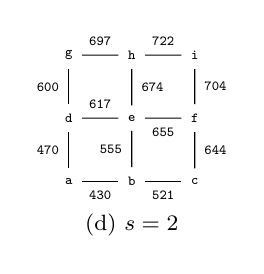
\begin{tikzpicture}[scale = 0.8]
\def\dx{0} 
\def\dy{0} 

\node[font=\bf] (a) at (\dx, \dy) {\tiny \texttt{a}};
\node[font=\bf] (b) at (\dx + 1, \dy) {\tiny \texttt{b}};
\node[font=\bf] (c) at (\dx + 2, \dy) {\tiny \texttt{c}};
\node[font=\bf] (d) at (\dx, \dy + 1) {\tiny \texttt{d}};
\node[font=\bf] (e) at (\dx + 1, \dy + 1) {\tiny \texttt{e}};
\node[font=\bf] (f) at (\dx + 2, \dy + 1) {\tiny \texttt{f}};
\node[font=\bf] (g) at (\dx, \dy + 2) {\tiny \texttt{g}};
\node[font=\bf] (h) at (\dx + 1, \dy + 2) {\tiny \texttt{h}};
\node[font=\bf] (i) at (\dx + 2, \dy + 2) {\tiny \texttt{i}};


\draw (a) edge[] node[anchor = north, font=\bf] {\tiny \texttt{430}} (b);
\draw (a) edge[] node[anchor = east, font=\bf]  {\tiny \texttt{470}} (d);
\draw (b) edge[] node[anchor = north, font=\bf] {\tiny \texttt{521}} (c);
\draw (b) edge[] node[anchor = east, font=\bf]  {\tiny \texttt{555}} (e);
\draw (d) edge[] node[anchor = east, font=\bf] {\tiny \texttt{600}} (g);
\draw (d) edge[] node[anchor = south, font=\bf]  {\tiny \texttt{617}} (e);
\draw (c) edge[] node[anchor = west, font=\bf]  {\tiny \texttt{644}} (f);
\draw (e) edge[] node[anchor = north, font=\bf] {\tiny \texttt{655}} (f);
\draw (e) edge[] node[anchor = west, font=\bf]  {\tiny \texttt{674}} (h);
\draw (g) edge[] node[anchor = south, font=\bf] {\tiny \texttt{697}} (h);
\draw (f) edge[] node[anchor = west, font=\bf]  {\tiny \texttt{704}} (i);
\draw (h) edge[] node[anchor = south, font=\bf] {\tiny \texttt{722}} (i);
\node at (1, -0.7) {\footnotesize (d) $s = 2$};
\end{tikzpicture} 
\end{tabular}
\end{center}

\caption{First two iterations of the execution of the algorithm on a 3 by 3 grid.}
\label{fig:ecmpfree}
\end{figure}

Figure \ref{fig:ecmpfree} shows the execution of the algorithm on a $3 \times 3$
grid. Figure \ref{fig:ecmpfree}(a) displays the initial prime numbers associated
to each edge, and Figure \ref{fig:ecmpfree}(b) conveys the result of computing
$\overline{\ln}^0$ on these numbers. Note that there is still ECMP (in blue), so
we iterate. Figure \ref{fig:ecmpfree}(c) reports the result of the second
iteration, using $\overline{\ln}^1$: There is still ECMP. Finally, 
Figure \ref{fig:ecmpfree}(d) shows the last iteration with $\overline{\ln}^2$: There is no more ECMP.

In practice, we cannot configure weights that are larger than $65535$, so we
stop our algorithm before this threshold is reached. This may leave some ECMP,
but our experiments show that the remaining ECMP is likely zero or negligible in
few corner cases. We ran the algorithm on all 243 connected topologies in the
Topology Zoo \cite{Knight_Zoo:2011} and the Rocketfuel \cite{rocketfuel-ton04}
topologies. The average number of iterations (value of $s$) was $1.16$ with
maximum value $4$. Only one instance, namely \texttt{SwitchL3} from the Topology Zoo
still had ECMP after the execution of our algorithm. In that topology, only $1 \%$ of
source-destination pairs had ECMP.

To implement this algorithm, we need to be able to find the first $m$ prime numbers. We can find these by iterating over the integers $2, 3, 5, 7, 9, \ldots$
and using any primality test algorithm to check which ones are prime numbers. The Prime number theorem \cite{cormen} %page 888 theorem 31.37
tells us that the $m$-th prime number is close to $m \ln(m)$ so we find them in a small number of steps.

\subsection{Dealing with link bundles}

Several physical cables between the same pair of nodes can be aggregated into a single logical (IGP) link.
In those cases, we cannot avoid multi-path routing, not even setting appropriate IGP weights in the monitoring topology.
%, we compute the IGP weights by considering each link bundle as a single link.
However, in order to monitor each physical cable, we need to explicitly represent all cables in a bundle and the corresponding multi-path routing.
We therefore derive a graph model of the monitoring topology.
We start from the IGP graph.
Then, for each link between $u$ to $v$ with several physical cables, we remove $(u,v)$ from our model; Moreover, for every physical cable in $(u,v)$, we add one fake node $f$ and two edges $(u,f)$ and $(f,v)$ and set their costs so that their sum is equal to the IGP cost $w(u,v)$.
%to the model of the monitoring topology, and split the weight of the link in two.
An example of this transformation is shown in Figure \ref{fig:bundle}.
Note that fake links intuitively translated into the need for using adjacency segments in our monitoring probes.
%Whenever a cycle crosses a fake node, it means that we have to use an adjacency segment
%to cross the correponding link.

\begin{figure}
\begin{center}
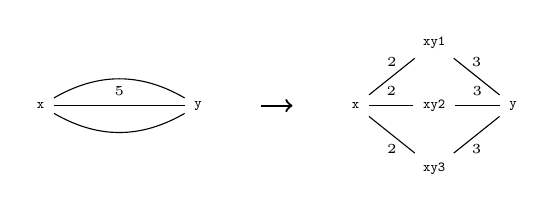
\begin{tikzpicture}
\node[font=\bf] (x) at (0, 0) {\tiny \texttt{x}};
\node[font=\bf] (y) at (2, 0) {\tiny \texttt{y}};
\draw (x) edge node[anchor = south, font=\bf] {\tiny $5$} (y);
\draw (x)  edge[bend left]  (y);
\draw (x)  edge[bend right] (y);

\draw[->, thick] (2.8, 0) -- (3.2, 0);

\node[font=\bf] (x) at (4, 0) {\tiny \texttt{x}};
\node[font=\bf] (y) at (6, 0) {\tiny \texttt{y}};
\node[font=\bf] (xy1) at (5, 0.8) {\tiny \texttt{xy1}};
\node[font=\bf] (xy2) at (5, 0) {\tiny \texttt{xy2}};
\node[font=\bf] (xy3) at (5, -0.8) {\tiny \texttt{xy3}};

\draw (x) edge node[anchor = south, font=\bf] {\tiny $2$} (xy1);
\draw (x) edge node[anchor = south, font=\bf] {\tiny $2$} (xy2);
\draw (x) edge node[anchor = north, font=\bf] {\tiny $2$} (xy3);
\draw (y) edge node[anchor = south, font=\bf] {\tiny $3$} (xy1);
\draw (y) edge node[anchor = south, font=\bf] {\tiny $3$} (xy2);
\draw (y) edge node[anchor = north, font=\bf] {\tiny $3$} (xy3);


\end{tikzpicture}
\end{center}
\caption{Link bundle transformation.}
\label{fig:bundle}
\end{figure}

\subsection{Computing the Cycle Cover}

From the graph model built as described in the previous section, we finally compute a cycle cover of the network.
Our algorithm is based on the two following observations:

\begin{enumerate}
 \item A shortest path can be represented by a single segment, provided that there
 is no ECMP.
 \item The set of shortest paths from one node to all other nodes in a graph forms
 a DAG. The longest paths in DAGs can be computed in linear
 time \cite{sedgewick2011algorithms}. %% page 661 proposition T
\end{enumerate}

The algorithm takes as input the weighted graph representing the monitoring
topology and a parameter $k$ specifying the maximum number of segments that
can be used for each cycle.

To find a cycle cover, we start by assigning a binary variable $u_{e}$ to each 
edge $e$ such that it has value $1$, if the edge is not yet covered by any cycle,
and $0$ otherwise. Then we call the \textit{cycle-finding algorithm} (described next)
until all edges are covered, that is, while $\sum_{e \in E} u_e > 0$. Every time
we find a cycle we set $u_e = 0$ for each edge of that cycle.

The cycle-finding algorithm is outlined in Figure \ref{figure:cycles}.
Starting from a source node $s$, it computes the longest path $\bar P$ (with
respect to the number of uncovered edges) in $\mathcal{D}_s$. After finding
$\bar P$, it then computes the longest path starting from the last node of $\bar
P$, and iterates on the latter found path for a given number of iterations
(depending on $k$). To avoid repeated edges in the built cycle, the algorithm
also keeps track of the edges traversed in previous iterations, and discards
paths (i) crossing already-traversed edges, or (ii) terminating in a node with
no path to $s$ disjoint from the already-traversed edges.
% (to close the cycle).
%so that we can close the cycle. 

\begin{figure}[htb]
\begin{center}
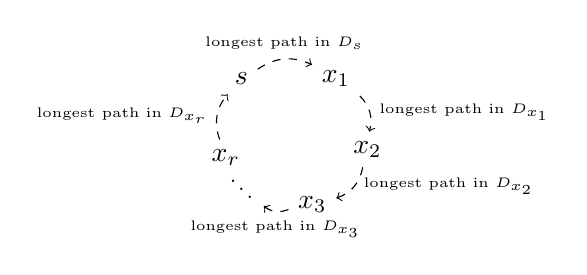
\begin{tikzpicture}[]
\node (a) at (0, 2.1) {$s$};

\node (b) at (1.2, 2.1) {$x_1$};


\draw[->, dashed] (a) edge[bend left] node[anchor = south] {\tiny longest path in $D_s$} (b);

\node (c) at (1.6, 1.2) {$x_2$};
\draw[->, dashed] (b) edge[bend left] node[anchor = west] {\tiny longest path in $D_{x_1}$} (c);

\node (d) at (0.9, 0.5) {$x_{3}$};
\draw[->, dashed] (c) edge[bend left] node[anchor = west] {\tiny longest path in $D_{x_2}$} (d);


\node[font=\bf] (e) at (0, 0.8) {\tiny $\ddots$};


\draw[->, dashed] (d) edge[bend left] node[anchor = north] {\tiny longest path in $D_{x_{3}}$} (e);

\node (f) at (-0.2, 1.1) {$x_{r}$};
\draw[->, dashed] (f) edge[bend left] node[anchor = east] {\tiny longest path in $D_{x_{r}}$} (a);
\end{tikzpicture}
\end{center}
\caption{Cycle construction outline}
\label{figure:cycles}
\end{figure}

\smallskip

The pseudocode of the cycle-finding algorithm is given in Algorithm
\ref{algo:findCycle}. The input is the graph $G$ of the monitoring topology, the
shortest path DAG $D$ computed on $G$, the node $source$ from which probes will
be sent and the segment budget $k$. We maintain the current node (corresponding
to the $x_i$'s in Figure \ref{figure:cycles}), the set of forbidden edges
$\mathcal{F}$ to avoid repeating edges, the binary variables $u$ indicating
whether an edge has already been covered and the cycle itself.
%
We use an algorithm \textsf{DAGLongestPath} that receives as input a shortest path DAG, a 
starting node $x$, the variables $u$ to use as path costs, the remaining segment budget
and the forbidden edges. It outputs the set of all the longest paths from the starting node
to the other nodes in the graph. For each of those paths, it provides a tuple
$(\textit{ending node}, \textit{path}, \textit{number of segments})$. Paths are
sorted by decreasing number of uncovered edges. In the case of
ties, they are broken by the number of uncovered edges in the DAG of the ending
node (the more the better). This ensures that if all the edges of a DAG are
covered we go to a node that is adjacent to an uncovered edge.
From this set of solutions, we select the best one that has a path to the
source with the remaining segment budget (lines 10-18).
Finally, we close the cycle by finding a path from the last node to the starting
node (if they differ). The last step is always possible since we only choose nodes
that have a path to $s$ as $x_i$ nodes.

\begin{algorithm}[htbp]
\small
\caption{\textsf{FindCycle}$\left( G, \mathcal{D}, \textit{source}, k \right)$}
\begin{algorithmic}[1]
\STATE $\textit{cur} \gets \textit{source}$
\STATE $\mathcal{F} \gets \emptyset$
\STATE $u_e \gets 1$ \textbf{forall} $e \in E(G)$
\STATE $\textit{cycle} \gets \textit{null}$
\STATE $S_1 \gets \textsf{DAGLongestPath}(\mathcal{D}, \textit{cur}, u, k, \mathcal{F})$
\WHILE{$|S_1| > 0$}
  \STATE $(\textit{next}, \textit{path}, \textit{nseg}) \gets (\textbf{null}, \textbf{null}, \textbf{null})$
  \WHILE{$|S_1| > 0$  \textbf{and} $\textit{next} = \textbf{null}$}
    \STATE $(x, p, s) \gets S_1.\textsf{RemoveBest}()$
    \STATE $S_2 \gets \textsf{DAGLongestPath}(\mathcal{D}, \textit{x}, u, k - s, \mathcal{F} \cup E(p))$
    \IF{$|S_2| > 0$}
      \STATE $(\textit{next}, \textit{path}, \textit{nseg}) \gets (x, p, s)$
    \ENDIF
  \ENDWHILE
  \IF{$\textit{next} \neq \textbf{null}$}
    \STATE $k \gets k - \textit{nseg}$
    \STATE $\mathcal{F} \gets \mathcal{F} \cup E(\textit{path})$
    \STATE $\textit{cur} \gets \textit{next}$
    \STATE $u_e \gets 0$ \textbf{forall} $e \in E(\textit{path})$
    \STATE $\textit{cycle} \gets \textit{cycle}.\textsf{Append}(\textit{path})$
    \STATE $S_1 \gets \textsf{DAGLongestPath}(\mathcal{D}_{\textit{cur}}, \textit{cur}, u, k, \mathcal{F})$
  \ENDIF
\ENDWHILE
\IF{$\textit{cycle}.\textsf{Last()} \neq \textit{source}$}
  \STATE $S_1 \gets \textsf{DAGLongestPath}(\mathcal{D}_{\textit{cur}}, \textit{cur}, u, k, \mathcal{F})$
  \STATE $(x, p, s) \gets S_1.\textsf{RemoveBest}()$
  \STATE $\textit{cycle} \gets \textit{cycle}.\textsf{Append}(\textit{path})$
\ENDIF
\RETURN $\textit{cycle}$
\end{algorithmic}
\label{algo:findCycle}
\end{algorithm}

The algorithm \textsf{DAGLongestPath} works in a similar fashion as the standard
dynamic programming algorithm for computing longest paths in directed acyclic
graphs \cite{sedgewick2011algorithms}. We extended it to also compute the number
of segments needed in the path. It does so by using the shortest path DAGs given
as input to check for ECMP. For all ECMP cases, it decreases the current segment
budget (since a new segment is needed). The time complexity of
\textsf{DAGLongestPath} is $O(E \cdot k)$.
%Due to space limitation we do not include the description of this
%algorithm.

\subsection{Segmenting Cycles}

% \hrule
% 
% \ed{sv: integrate the following two sentences among guarantees of the procedure (maybe we can move all proofs plus this kind of observation in a separate subsection?).}
% In the case of ECMP-free weights, after $r$ iterations we know that the cycle we obtain 
% has a simple segmentation with at most $r$ segments. Moreover, in this case we know
% that if $k \geq 3$ the algorithm will always find a solution since any edge can be covered using at most $3$
% segments. 
% 
% \hrule

Once we have a cycle cover of the graph, we need to be able to represent them as
a list of segments. Our \textit{segmenting algorithm} computes ECMP-free
segmentations so that $(i)$ it uses adjacency segments only when any other
segmentation would also use one, and $(ii)$ it minimizes the remaining node
segments. Those two properties imply that if the input path admits a simple
segmentation, our algorithm will produce a minimal simple segmentation.
%%%%%
\begin{algorithm}
\small
\caption{\textsf{MinSegECMP}$((x_1, x_2, \ldots, x_n), \mathcal{D})$}
\begin{algorithmic}[1]
\STATE $r \gets 1$
\STATE $S \gets \langle \rangle$
\FOR{$i \gets 1$ \textbf{to} $n - 1$}
 \IF{$(x_i, x_{i + 1}) \notin E(D_r)$}
%   \STATE{{\color{gray} \# edge $(x_i, x_{i + 1})$ not in dag $D_r$}}
   \IF{$d^-_{D_{x_i}}(x_{i + 1}) = 1$}
%      \STATE{{\color{gray} \# edge $(x_i, x_{i + 1})$ is in dag $D_{x_i}$ and no multipath}}
      \STATE $S \gets S + x_i$
      \STATE $r \gets x_i$
   \ELSE
%      \STATE{{\color{gray} \# edge $(x_i, x_{i + 1})$ is in no dag}}
      \STATE $S \gets S + \langle x_i, (x_i, x_{i + 1}) \rangle$
      \STATE $r \gets x_{i + 1}$
   \ENDIF
 \ELSIF{$d_{D_r}^-(x_{i + 1}) > 1$}
%   \STATE{{\color{gray} \# edge $(x_i, x_{i + 1})$ is in dag but multipath in $D_r$}}
   \IF{$d^-_{D_{x_i}}(x_{i + 1}) > 1$}
%     \STATE{{\color{gray} \# multipath also in $D_{x_i}$}}
     \STATE $S \gets S + \langle x_i, (x_i, x_{i + 1}) \rangle$
     \STATE $r \gets x_{i + 1}$
   \ELSE
     \STATE $S \gets S + x_i$
     \STATE $r \gets x_i$
   \ENDIF
 \ENDIF
\ENDFOR
\RETURN $S$
\end{algorithmic}
\label{algo:segECMP}
\end{algorithm}

The pseudo-code of the algorithm is reported in Algorithm \ref{algo:segECMP}. It
receives as input a path $p$ and a shortest path DAG $D$ and outputs an
ECMP-free segmentation of $p$. Its complexity is linear with respect to the
length of $p$.
%However, the pre-computation of the shortest path DAGs requires
%$O(n^3)$ using Floyd-Warshall's algorithm \cite{cormen}.
%Note also that the algorithm does not
%need to know all shortest path DAG's, only the ones that correspond to segments in the output so if
%we only want to segment one path it is better to compute the DAG's as needed. In this case the
%complexity is $O(n + k \cdot E \log(V))$ where $k$ is the number of segments in the output.
%However, since we also use the shortest path DAG's in the cycle finding algorithm, we find
%it easier to just precompute them at the start.

We now show that the algorithm produces a valid segmentation.

% \begin{lemma}
% Algorithm \ref{algo:segECMP} computes an ECMP-free segmentation of the
% input path.
% \end{lemma}
% 
% \begin{proof}
% Let $p = (x_1, x_2, \ldots, x_n)$ be the input path and $\langle s_1, s_2, \ldots, s_k \rangle$ the output of the algorithm.
% It is clear that each $s_i \in S(p)$ by the way the algorith is defined. Everytime we add a segment it is either a pair $(x_i, x_i)$
% or an edge $(x_i, x_{i + 1})$ of the path $p$. 
% %Also, by the order in which we loop over $p$, the segmentation $S$ clearly is ordered relative to $p$.
% 
% Let $(x_i, x_{i + 1})$ be an edge of $p$. We want to show that it belongs to $G_S$ so that $p$ is a sub-path of $G_S$.
% If $(x_i, x_{i + 1}) = s_j$ for some $j$ there is nothing to show. Otherwise, 
% let $s_j$ be the last segment that ends before or at $x_i$. Since $(x_i, x_{i + 1})$ is not a adjacency segment of $S$,
% we know that $\underline{s}_{j + 1}$ does not come before $x_{i + 1}$. By the way the algorithm is defined, each edge in $p$ 
% from $\underline{s}_j$ to $\underline{s}_{j + 1}$ belong to $\mathcal{D}_{\underline{s}_j}$. 
% We just saw that these contain the edge $(x_i, x_{i + 1})$ so it must belong to $G_S$.
% % If $s_i = (x_i, x_{i + 1})$ with $x \neq y$ then $s_i$ must have been added either on line 12 or line 19. In either case $y = x + 1$
% % and $(x, x + 1) \in E(p)$. On the other hand, if $s_i = (x, x)$ then clearly $x \in V(p)$ since $x$ loops exactly over those
% % elements. By the order in wich we loop over the elements in line 3 it is also clear that $s_1 < s_2 < \ldots < s_k$.
% % 
% % Let $(x, x + 1) \in E(p)$. We want to show that this edge belongs to $E(G_S)$.
% % If $(x, x + 1) = s_i$ for some $i$ then there is nothing to show. Otherwise, the same argument as in the proof
% % of Lemma \ref{lemma:simple_seg} applies.
% % 
% % It remains to show that $S$ is ECMP-free. By definition, if $G_S$ is not a path then there must
% % be some $i$ such that $\textit{path}(s_i)$ has at least two elements. Therefore the in-degree
% % of $s^0_{i + 1}$ in the DAG rooted at $s^1_{i}$ is at least two. This means that in the loop
% % when $x = s^0_{i + 1} - 1$ we must enter the if at line 15 so either $(s^0_{i + 1} - 1, s^0_{i + 1} - 1)$ or $(s^0_{i + 1} - 1, s^0_{i + 1})$
% % is an element in $S$. Both cases are impossible since each would give a segment in $S$ between
% % $s_i$ and $s_{i + 1}$.
% \end{proof}

\begin{lemma}
Let $\textit{seg}_i$ and $\textit{seg}_{i + 1}$ be two consecutive elements in the segment list produced
by Algorithm \ref{algo:segECMP}. Suppose that $\textit{seg}_i $ and $\textit{seg}_{i + 1}$ are both
node segments.
Then there is a unique shortest path from $\textit{seg}_i$ to $\textit{seg}_{i + 1}$.
\end{lemma}

\begin{proof}
Suppose that there exist two shortest paths from $\textit{seg}_i$ to $\textit{seg}_{i + 1}$.
Then the in-degree of $\textit{seg}_{i + 1}$ in the shortest path DAG rooted at $\textit{seg}_i$
is larger than one. But, in this case, the algorithm would have either produced an adjacency segment on the edge
of the input path ending at $\textit{seg}_{i + 1}$ (on line 19) or a node segment at the last node of $p$ before
node $\textit{seg}_{i + 1}$ (on line 22). In either case, this contradicts the fact that $\textit{seg}_{i + 1}$
is the element after $\textit{seg}_i$ in the segment list.
\end{proof}

When $\textit{seg}_i $ is an adjacency segment and $\textit{seg}_{i + 1}$ is a node segment,
a similar argument applies. In the other cases there is nothing to show.
This gives the following corollary.

\begin{corollary}
The segmentations produced by Algorithm \ref{algo:segECMP} are ECMP-free.
\end{corollary}

Now we establish that some adjacency segments must be in any ECMP-free segmentation
and that those are the only adjacency segments present in the segmentation produced by
Algorithm \ref{algo:segECMP}.

\begin{lemma}
Let $p = (x_1, x_2, \ldots, x_n)$ be a path on a graph $G$. 
If the segment list of $p$ produced by Algorithm \ref{algo:segECMP} possesses an adjacency segment $(x_i, x_{i + 1})$
then the segment list of any ECMP-free segmentation of $p$ possesses this adjacency segment.
\end{lemma}

\begin{proof}
Algorithm \ref{algo:segECMP} produces adjacency segments in two cases: The edge $(x_i, x_{i + 1})$ does not belong to any
shortest path DAG or there exists a shortest path from $x_i$ to $x_{i + 1}$ different than $(x_i, x_{i + 1})$.
It is obvious that any segmentation contains adjacency segments on all edges
that do not belong to any shortest path since it is the only way we can cross them. In the latter case,
if a segmentation passes through the edge via a shortest path $p$, then $p$ cannot be a unique shortest path since
its last edge is $(x_i, x_{i + 1})$. We can get another one by removing the node $x_{i + 1}$ from $p$
and concatenating the result with the other shortest path from $x_i$ to $x_{i + 1}$.
%We thus focus 
% on the second case.
% 
% Let $p'$ be a shortest path from $x_i$ to $(x_{i + 1})$ different from $(x_i, x_{i + 1})$. 
% Let $S  = \langle \textit{seg}_1, \ldots, \textit{seg}_k \rangle$ be any segment list of any ECMP-free segmentation of $p$ and suppose that
% $(x_i, x_{i + 1})$ is not in it. Let $s_i$ be the last segment that ends before or at node $x_i$. Then
% $(\overline{s}_i, \overline{s}_i + 1, \ldots, x_i, x_{i + 1})$ and $(s^1_i, s^1_i + 1, \ldots, x_i)$ concatenated by $p'$
% are both shortest pahts, thus, elements of $\textit{path}(s_i)$. Therefore $S$ is not ECMP-free since $G_S$ is not a path.
\end{proof}

The next lemma shows that Algorithm \ref{algo:segECMP} minimizes the remaining node segments.

\begin{lemma}
\label{lemma:min_seg_ecmp}
Let $p = (x_1, x_2, \ldots, x_n)$ be a path in a graph $G$ and let $S = s_1 \oplus s_2 \oplus \ldots \oplus s_k$ be the segmentation corresponding to the
segment list produced by Algorithm \ref{algo:segECMP}. 
Let $S'$ be any ECMP-free segmentation of $p$ having the exact same set of adjacency segments. Then, for each $i$ such that $s_i \in \textit{Sp}(G)$,
there exists a node in $s_i$ that is a node segment in the segment list of $S'$.
\end{lemma}

\begin{proof}
Suppose that no node in $s_i$ is a node segment on the segment list of $S'$. Then, since both segmentations have the same adjacency
segments, no edge of $s_i$ is an adjacency segment in the segment list of $S'$. Therefore,
there must be a shortest path $s'$ starting before (or at) $\textit{first}(s_i)$ in $S'$. This contradicts the fact that
$s_i$ was produced by Algorithm \ref{algo:segECMP} in the first place because when $\textit{last}(s_i)$ was added to the segment list,
the condition on line 4 must have been false meaning that the edge is not a shortest path edge in the shortest path DAG of $\textit{first}(s_i)$. Thus  that edge
cannot also be  a shortest
path edge in the $\textit{first}(s')$, since the node does not come after $\textit{first}(s_i)$. This contradicts the fact that $s'$ is a shortest path.
% Let $i$ be such that $s_i$ is a node segment. If $i = 1$ and $\underline{s}_i = 1$ or $i = k$ and $\overline{s}_i = n$ then, since $s_i$ is a node segment, it must
% also be a node segment in $S'$. We can therefore assume that $i \in \{2, 3, \ldots, k - 1 \}$. Then if $S'$ has no node segment
% between $\overline{s}_{i - 1}$ (exclusive) and $\underline{s}_{i}$ (inclusive) it means that the sub-path of $p$ from
% $\overline{s}_{i - 1}$ to the first node, say $z$, of $p$ after $\underline{s}_i$ is a shortest path by construction (notice that by hypothesis both segmentations
% contain the same adjacency segments and thus none of them has an adjacency segment in this sub-path).
% 
% This contradicts the fact that $s_i$ was produced in the first place since this only happens when the
% edge $(\underline{s}_{i}, z)$ does not belong to the shortest path dag of $s_{i - 1}$.
\end{proof}

A corollary of Lemma \ref{lemma:min_seg_ecmp} is the following proposition,
stating that Algorithm \ref{algo:segECMP} uses the strictly-minimum number of
adjacency segments and also minimizes node segments.
%That is, the following proposition holds.
%In other words, for every node segment in our segmentation we can find one
%in any other segmentation using the same set of adjacency segments.
%We choose to restrict ourselves to the
%strict minimum of adjacency segments. Indeed, they are more expensive than node segments since we need to specify two labels for an adjacency segment.
%This is summarized in the next proposition.

\begin{proposition}
Algorithm \ref{algo:segECMP} computes an ECMP-free segmentation of the input path such that: (1) it contains an adjacency segment if 
and only if all segmentations of the input path contain that adjacency segment; (2) the number of node segments used is minimal.
\end{proposition}

%However do not have the guarantee that we will be able to cover the entire network anymore for
%a given $k$ as it can happen that some edges require too many segments to be reached. One possible
%way to overcome this it by using multiple sources, when we cannot cover more edges from the current
%source then we choose another one. This m eans that several there will be more than one node
%in the network doing experiments.


% 
% The formal description of the algorithm is given
% in Algorithm \ref{algo:cycle_cover}.
% 
% \begin{algorithm}
% \caption{\textsf{CycleCover}$(G, S, K)$}
% \begin{algorithmic}[1]
% \STATE{{\color{gray} // compute the shortest path dag's}}
% \FOR{$i = 1$ \textbf{to} $|V|$}
%   \STATE $\mathcal{D}_i \gets \textsf{ShortestPath}(i).dag$
% \ENDFOR
% \STATE remove all edges of $G$ that do not belong to a shortest path dag
% \STATE $C \gets \emptyset$
% \WHILE{$w(G) > 0$}
%   \STATE let $s \in S$ be a node that maximizes $w(\mathcal{D}_s)$
%   \STATE $c \gets \textsf{FindCycle}(G, K, s, \mathcal{D}_1, \ldots, \mathcal{D}_n)$
%   \STATE \textbf{forall} $e \in E(c)$, $w(e) \gets 0$
%   \STATE $C \gets C \cup \{ c \}$
% \ENDWHILE
% \RETURN $C$
% \end{algorithmic}
% \label{algo:cycle_cover}
% \end{algorithm}
% 
% \begin{algorithm}
% \caption{\textsf{FindCycle}$(G, K, s, \mathcal{D}_1, \ldots, \mathcal{D}_n)$}
% \begin{algorithmic}[1]
% \STATE $cycle \gets ()$
% \STATE $cur \gets s$
% \STATE $w \gets \mathbf{1}_E$
% \STATE $f \gets \emptyset$
% \STATE $over \gets \textbf{false}$
% \WHILE{$i \leq K$ \textbf{and} \textbf{not} $over$}
%   \STATE $LP \gets \textsf{LongestPath}(\mathcal{D}_{cur}, w, f)$
%   \STATE{{\color{gray} // get the set of end nodes of longest paths}}
%   \STATE $X \gets LP.\textsf{endnodes}$
%   \STATE{{\color{gray} // sort $X$ so that $w(\mathcal{D}_{x_j}) \geq w(\mathcal{D}_{x_{j + 1}}$ )}}
%   \STATE $\textsf{SortByDagWeight}(X)$
%   \STATE $j \gets 1$
%   \STATE{{\color{gray} // check if there is a path from $x_j$ to $s$ in $\mathcal{D}_{x_j}$ avoiding edges in $f \cup E(p))$}}
%   \STATE{{\color{gray} // where $p = LP.\textsf{path}(x_j)$ is the longest path from $cur$ to $x_j$}}
%   \WHILE{$j \leq |X|$ \textbf{and} \textbf{not} $\textsf{Connected}(x_j, s, \mathcal{D}_{x_j}, f \cup E(LP.\textsf{path}(x_j)))$}
%     \STATE $j \gets j + 1$
%   \ENDWHILE
%   \IF{$j > |X|$}
%     \STATE $over \gets \textbf{true}$
%   \ELSE
%     \STATE{{\color{gray} // update data with new path}}
%     \STATE $p \gets LP.\textsf{path}(x_j)$
%     \STATE \textbf{forall} $e \in E(p)$, $w(e) \gets 0$
%     \STATE $f \gets f \cup E(p)$
%     \STATE $cycle \gets cycle + p$
%     \STATE $cur \gets x_j$
%     \STATE $i \gets i + 1$
%   \ENDIF   
% \ENDWHILE
% \STATE{{\color{gray} // come back to $s$}}
% \STATE $p \gets \textsf{LongestPath}(\mathcal{D}_{cur}, w, f).\textsf{path}(p)$
% \STATE $w(e) \gets 0$ \textbf{forall} $e \in E(p)$
% \STATE $cycle \gets cycle + p$
% \RETURN $cycle$
% \end{algorithmic}
% \label{algo:find_cycle}
% \end{algorithm}
% 
% In line $11$ in Algorithm \ref{algo:find_cycle}, when we sort the set $X$ we do not need to compute $w$ on all the dag's of elements of $X$.
% Instead we keep a data structure that keeps for each edge, the set of shortest path dag's that contain it.
% Then everytime we select a new path we just go over all edges in the path an decrement the value of each
% dag that contains the $e$ by $1$. This allows $O(1)$ comparisons.


